% \documentclass[a4paper]{article}
% \usepackage[ngerman]{babel}
% \usepackage[utf8]{inputenc}
% \usepackage[top=2.5cm,bottom=1.75cm,right=2cm,left=2.3cm]{geometry}
% \usepackage{wrapfig}
% \usepackage{floatflt}
% \usepackage{subfigure}
% \usepackage{graphicx}
% \usepackage[colorlinks=true,linkcolor=black,bookmarksnumbered=true,breaklinks=true,pdfstartview=FitH]{hyperref}
% 
% \title{\textbf{Praktikum 12} \\ ~ \\Bestimmung des Planck'schen Wirkungsquantums}
% 
% \author{Michael Kopp}
% 
% \date{14. Februar 2008}
% 
% \begin{document}
% 
% \maketitle
% \tableofcontents



\section{Versuch}

Zur Bestimmung des \emph{\textsc{Planck}'schen Wirkungsquantums} $h$ benötigen wir die Wellenlänge $\lambda$ bzw. Frequenz $f$ untersuchten Lichts sowie die damit transportierte Energie $W$. Über den Zusammenhang $W = h \cdot f$ lässt sich dann das \textsc{Planck}'sche Wirkungsquantum errechnen:
\begin{equation}
   h = \frac{W}{f}
   \label{eq_hwf}
\end{equation}
Wir verwenden in unseren Versuchen Leuchtdioden. Einerseits weil ihr Licht weitgehend \emph{monochromatisch} ist, andererseits aber auch, weil die abgestrahlte Energie dabei leicht bestimmt werden kann.







\subsection{Bestimmung der Abgestrahlten Energie}

Bei Leuchtdioden muss jedes Elektron energetisch vom Valenzband auf ein Leitungsband angehoben werden. Von dort kann es wieder zurückfallen und bei diesem Zurückfallen ein Photon emittieren. Entscheidend ist dabei, dass ein Elektron eine bestimmte Mindestenergie braucht, um den \textit{Bandwechsel} vollziehen zu können. Diese Mindestenergie ist dann auch genau die Energie, die es wieder abgibt, wenn es vom energetisch höheren Leitungsband wieder in das Valenzband zurückfällt -- unabhängig davon, mit wie viel Energie \textit{hochgehievt} wurde.

Bestimmt man nun also die Energie, die zum Wechsel vom Valenz- ins Leitungsband von jedem Elektron aufgebracht werden muss, so ist diese Energie gleich der, die ein Elektron beim Übergang vom Leitungs- ins Valenzband in Form eines Photons abgibt. Wird an eine Diode die Spannung $U$ angelegt, so erhält ein einzelnes Elektron die Energie
\begin{equation}
   W = U \cdot e
   \label{eq_wue}
\end{equation}
Um nun die Energie zum Bandwechsel zu bestimmen, bestimmt man die \emph{kleinste mögliche} Spannung $U$, bei der Elektronen den Wechsel ins Leiterband schaffen. Dies äußert sich dann dadurch, dass die Diode überhaupt erst Strom leitet -- unterhalb dieser Spannung sitzen die Elektronen ja im Valenzband "`fest"'. Aus diesem Grund wird diese Spannung auch als \emph{Durchlassspannung} $U_D$ bezeichnet.

Praktisch verwendet man den in Abb. \ref{abb_schaltung} skizzierten Aufbau. Dabei wird eine Leuchtdiode über einen Widerstand in Durchlassrichtung mit einer regelbaren Spannungsquelle verbunden. Der fließende Strom wird gemessen ebenso wie die Spannung, die zwischen den Enden der Leuchtdiode -- und damit auch innerhalb der Leuchtdiode -- besteht. Die Spannung wird nun schrittweise erhöht und die Werte für Stromstärke und Spannung Tabelliert.


\begin{figure}
   \centering
   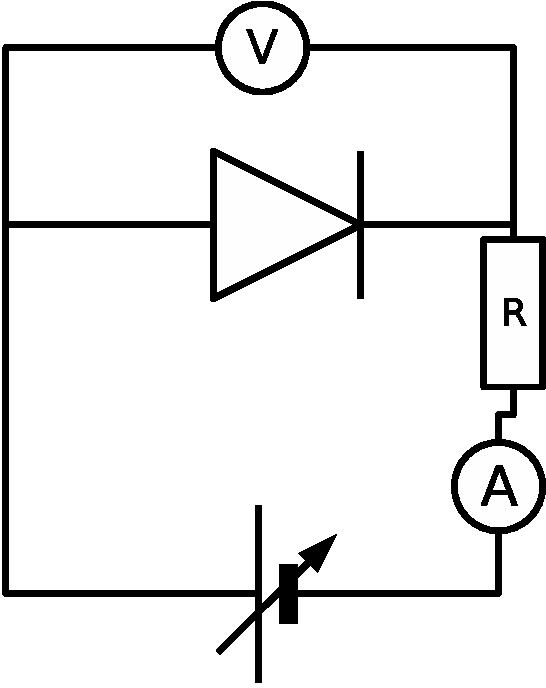
\includegraphics[width=0.4\textwidth]{praktika/mat_praktika/schaltung01}
   \caption{Aufbau um eine $I$-$U$-Kennlinie von Leuchtdioden aufzunehmen.}
   \label{abb_schaltung}
\end{figure}








\subsection{Bestimmung der Wellenlänge}

Zur Bestimmung der Wellenlänge von Licht verwendet man die Beugung von Licht am Gitter. Eine Leuchtdiode sendet als Lichtquelle Licht aus, welches in einem Gitter gebeugt wird. \emph{Hinter} dem Gitter steht ein Beobachter. Auf seine Netzhaut fällt das gebegte Licht. Nimmt das Auge ein Maximum wahr, so geht das Gehirn davon aus, dass das Licht des Maximums sich senkrecht zur Gitterebene ausgebreitet hat. Das Gehirn spiegelt dem Beobachter also vor, er sähe zwei erste Maxima links und rechts\footnote{Wenn die Gitterstriche senkrecht verlaufen.} der Lichtquelle. In Abb. \ref{abb_wellenlaenge} ist dies im unteren Teil zu sehen.

Um nun aber die Wellenlänge von Licht bestimmen zu können, benötigt man theoretisch ein Maximum bekannter Ordnung auf einem Schirm. Der Schrim ist in diesem Falle unser Gehirn. Unterhalb der LED wird eine Schiene befestigt, auf der Klammern rechts und links befestigt sind. Diese werden so gestellt, dass sie die Maxima 1. Ordnung seitlich "`berühren"'. So kann man den Abstand zwischen den beiden Maxima festhalten.

Als Distanz $a$ vom Gitter zum Schirm im klassischen Versuch wird in diesem Aufbau die Distanz $a_2$ vom Gitter zu der Schine mit den Klammern verwendet. Hier kann man den Abstand $d_1$ zwischen zwei Maxima 1. Ordnung abmessen -- der Abstand vom Maximum 0. Ordnung zu einem 1. Ordnung beträgt somit $\frac{d_1}{2}$. Dieses Licht wird also um den Winkel $\alpha_1$ gebeugt:
\begin{equation}
   \alpha_1 = arctan \left ( \frac{d_1}{a} \right )
\end{equation}
Bei Licht darf man die \emph{\textsc{Fraunhofer}'sche Näherung} anwenden, weil $a_2 \gg g$ gilt. Somit ergibt sich für ein Maximum 1. Ordnung unter den Winkel $\alpha_1$ die Wellenlänge
\begin{equation}
   \lambda = g \cdot sin ( \alpha_1 ) =  g \cdot sin \left ( arctan \left ( \frac{d_1}{a} \right ) \right ) 
   \label{eq_wellenlaenge_berechnen}
\end{equation}



\begin{figure}
   \centering
   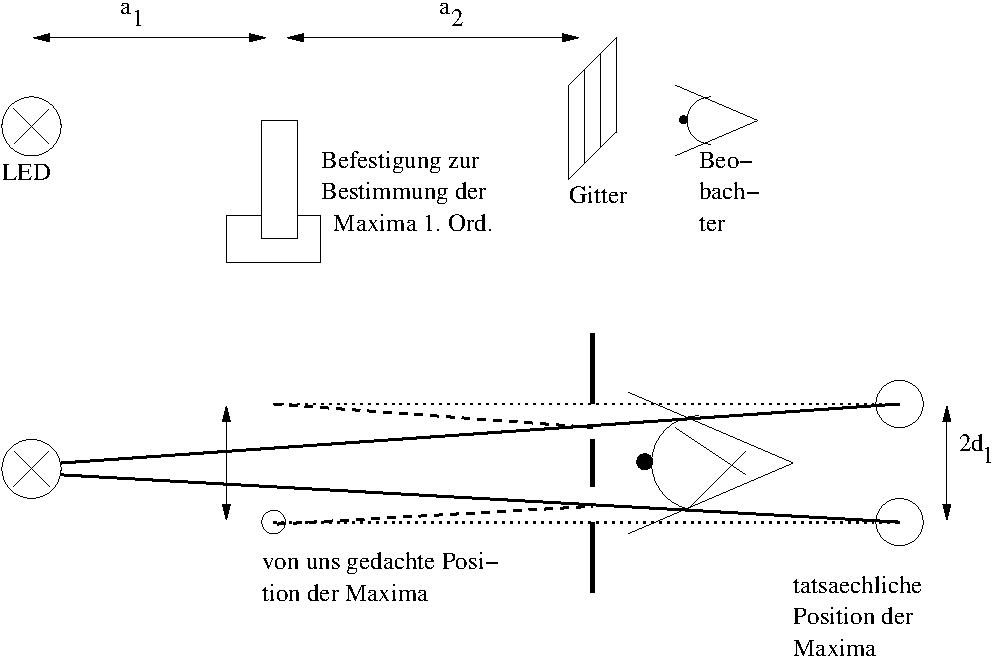
\includegraphics[width=\textwidth]{praktika/mat_praktika/aufbau_12}
   \caption{Versuchsaufbau zur Bestimmun der Wellenlänge von Licht}
   \label{abb_wellenlaenge}
\end{figure}






\section{Messwerte}


\subsection{Ermittlung der Durchschlagspannung}

Für verschiedene Leuchtdioden kamen wir auf die in Tabelle \ref{tab_messwerte} auf S. \pageref{tab_messwerte}zusammengestellten Ergebnisse. In Abb. \ref{abb_kennlinie} auf S. \pageref{abb_kennlinie} sind diese Werte zusammengefasst in Form von sog. \emph{I-U-Kennlinien}. In Tabelle \ref{tab_durchschlag} auf S. \pageref{tab_durchschlag} sind die einzelnen Durchschlagspannungen aufgelistet. %Die sich nach Formel \ref{eq_wue} ergebenden transportierten Energien sind hier ebenfalls eingetragen.


\begin{table}
\caption{Messwerte zur Bestimmung der Durchschlagspannung der einzelnen Leuchtdioden}\label{tab_messwerte}
\centering
\subtable[
Messwerte der blauen Leuchtdiode
]{
\begin{tabular}{l | l}
%~~~ # I  & ~~~ # U  \\
~~~ I [mA] & U [V]\\
\hline
~~~ 0  & ~~~ 0  \\
~~~ 0  & ~~~ 1.6  \\
~~~ 0.01  & ~~~ 1.64  \\
~~~ 1.18  & ~~~ 3.26  \\
~~~ 2.04  & ~~~ 3.34  \\
~~~ 2.98  & ~~~ 3.39  \\
~~~ 5.31  & ~~~ 3.47  \\
~~~ 6.92  & ~~~ 3.51  \\
~~~ 8.04  & ~~~ 3.54  \\
~~~ 10.18  & ~~~ 3.58  \\
~~~ 10.98  & ~~~ 3.59  \\
~~~ 12.05  & ~~~ 3.62  \\
~~~ 13.03  & ~~~ 3.63  \\
~~~ 13.51  & ~~~ 3.64  \\
~~~ 14.16  & ~~~ 3.65  \\
~~~ 15.02  & ~~~ 3.66  \\
~~~ 15.14  & ~~~ 3.66  \\
~~~ 17.37  & ~~~ 3.7  \\
\end{tabular}
}\label{tab_blau}
\subtable[
Messwerte der grünen Leuchtdiode
]{
\begin{tabular}{l | l}
%~~~ #I [mA]  & ~~~ U [V]  \\
~~~ I [mA] & ~~~~U [V]\\
\hline
~~~ 0  & ~~~ 0  \\
~~~ 0  & ~~~ 1.65  \\
~~~ 1.38  & ~~~ 1.85  \\
~~~ 3.31  & ~~~ 1.91  \\
~~~ 5.35  & ~~~ 1.96  \\
~~~ 7.5  & ~~~ 2  \\
~~~ 9.29  & ~~~ 2.03  \\
~~~ 10.6  & ~~~ 2.05  \\
~~~ 13.12  & ~~~ 2.09  \\
~~~ 14.7  & ~~~ 2.12  \\
~~~ 16.51  & ~~~ 2.14  \\
~~~ 18.5  & ~~~ 2.17  \\
\end{tabular}
}\label{tab_gruen}
\subtable[
Messwerte der gelben Leuchtdiode
]{
\begin{tabular}{l | l}
~~~ I [mA]  & ~~~ U [V]  \\
\hline
~~~ 0  & ~~~ 0  \\
~~~ 0  & ~~~ 1.52  \\
~~~ 0.1  & ~~~ 1.65  \\
~~~ 0.51  & ~~~ 1.71  \\
~~~ 1.66  & ~~~ 1.77  \\
~~~ 3.12  & ~~~ 1.82  \\
~~~ 3.35  & ~~~ 1.83  \\
~~~ 7.06  & ~~~ 1.91  \\
~~~ 7.94  & ~~~ 1.93  \\
~~~ 11.8  & ~~~ 2  \\
~~~ 15.03  & ~~~ 2.05  \\
~~~ 16.61  & ~~~ 1.98  \\
~~~ 19.8  & ~~~ 2.12  \\
\end{tabular}
}\label{tab_gelb}

\subtable[
Messwerte der roten Leuchtdiode
]{
\begin{tabular}{l | l}
~~~ I [mA]  & ~~~ U [V]  \\
\hline
~~~ 0  & ~~~ 0  \\
~~~ 0  & ~~~ 1.3  \\
~~~ 0.18  & ~~~ 1.46  \\
~~~ 1.43  & ~~~ 1.55  \\
~~~ 3.14  & ~~~ 1.58  \\
~~~ 7.16  & ~~~ 1.61  \\
~~~ 9.78  & ~~~ 1.62  \\
~~~ 11.75  & ~~~ 1.63  \\
~~~ 14.15  & ~~~ 1.64  \\
~~~ 16.25  & ~~~ 1.65  \\
~~~ 17.88  & ~~~ 1.65  \\
\end{tabular}
}\label{tab_rot}
\subtable[
Messwerte der infraroten Leuchtdiode
]{
\begin{tabular}{l | l}
~~~ I [mA]  & ~~~ U [V]  \\
\hline
~~~ 0  & ~~~ 0  \\
~~~ 0  & ~~~ 0.81  \\
~~~ 0.17  & ~~~ 0.95  \\
~~~ 0.67  & ~~~ 1.01  \\
~~~ 1.54  & ~~~ 1.04  \\
~~~ 2.57  & ~~~ 1.06  \\
~~~ 3.57  & ~~~ 1.08  \\
~~~ 5.71  & ~~~ 1.09  \\
~~~ 6.3  & ~~~ 1.1  \\
~~~ 8.18  & ~~~ 1.11  \\
~~~ 12.86  & ~~~ 1.13  \\
~~~ 13.95  & ~~~ 1.13  \\
~~~ 14.97  & ~~~ 1.14  \\
\end{tabular}
}\label{tab_ir}
\subtable[Durchschlagspannungen der einzelnen Leuchtdioden]{
\begin{tabular}{l l}
   Farbe der LED & $U_D$ [V]\\
   \hline
   Blau & 1,6  \\
   Grün  & 1,65\\
   Gelb & 1,52\\
   Rot & 1,3\\
   Infrarot & 0,81   \\
\end{tabular}\label{tab_durchschlag}}

\end{table}


\begin{figure}
   \centering
   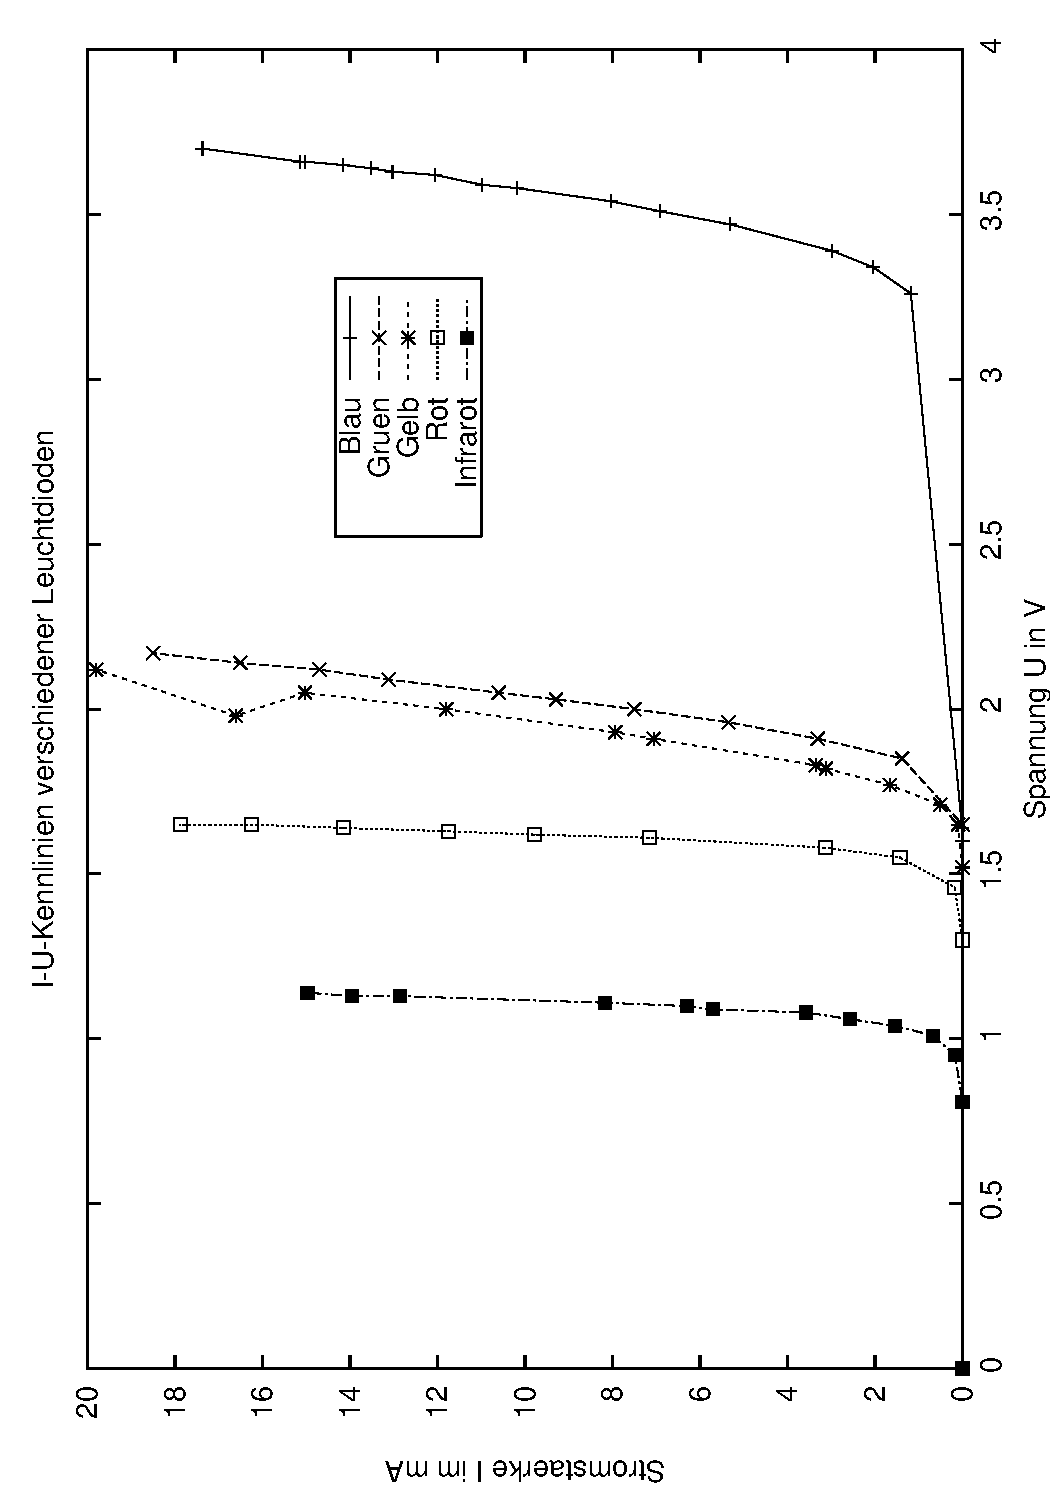
\includegraphics[height=\textwidth,angle=-90]{praktika/mat_praktika/plot01_01}
   \caption{Die Daten aus Tabelle \ref{tab_messwerte} in einem Schaubild zusammengefasst.}
   \label{abb_kennlinie}
\end{figure}








\subsection{Bestimmung der Wellenlänge}

Für unseren Aufbau gilt (nach Abb. \ref{abb_wellenlaenge}):

$a_2 = 0,80m = 80cm$

$g = 1 \cdot 10^{-5}$

Die Messwerte für die einzelnen Abstände sind in Tabelle \ref{tab_d_1} festgehalten.



\begin{table}[h]
   \centering
   \begin{tabular}{l l l}
   Farbe der LED & ~~~ $d_1$\\
   \hline
      Blau & ~~~ 8,6cm\\
      Grün & ~~~ 9,8cm\\
      Gelb & ~~~ 10,5cm\\
      Rot & ~~~ 11,4cm
   \end{tabular}
\caption{Messwerte zur Bestimmung der Wellenlänge der einzelnen LEDs}
\label{tab_d_1}
\end{table}







\section{Auswertung}

Für die einzelnen LEDs ergeben sich somit Energien (berechnet aus den Durchschlagspannungen aus Tab. \ref{tab_durchschlag} mit Gleichung \ref{eq_wue}) und Wellenlängen (berechnet aus der Lage der Maxima und Gleichung \ref{eq_wellenlaenge_berechnen}) wie sie in Tabelle \ref{tab_auswertung} festgehalten sind. Die Abweichung vom Literaturwert ist direkt dahinter angegeben -- für uns ergibt sich also eine Abweichung vom Literaturwert von durchschnittlich $-23,8\%$.




\begin{table}[h]
   \centering
   \begin{tabular}{l l l l l l}
      Farbe der LED & ~~~ $W$ [J]& ~~~ $\lambda$ [m]& ~~~ $f$ [Hz]& ~~~ $h$ [Js] & Abweichung\\
      \hline
      Blau & $2,56E-19$ & ~~~$5,37E-07$ & ~~~$5,59E+14$ & ~~~$4,59E-34$ & ~~~ $-3,08E-01$\\
      Grün & $2,64E-19$ & ~~~$6,11E-07$ & ~~~$4,91E+14$ & ~~~$5,39E-34$ & ~~~ $-1,88E-01$\\
      Gelb & $2,44E-19$ & ~~~$6,55E-07$ & ~~~$4,58E+14$ & ~~~$5,32E-34$ & ~~~ $-1,98E-01$\\
      Rot & $2,08E-19$ & ~~~$7,11E-07$ & ~~~$4,22E+14$ & ~~~$4,93E-34$ & ~~~ $-2,56E-01$
      
   \end{tabular}
   \caption{Die Messergebnisse aus der Bestimmung der abgestrahlten Energie und der Bestimmung der Wellenlänge werden hier zusammengesetzt und es wird das -- eigentlich gesuchte -- \textsc{Planck}'sche Wirkungsquantum errechnet.}
   \label{tab_auswertung}

\end{table}



\paragraph{Bestimmung von h näherungsweise aus einem f-D-Schaubild}


In Abb. \ref{abb_fu} auf S. \pageref{abb_fu} ist ein $f$-$U_D$-Diagramm für alle LEDs gezeichnet. Hier ist die Ablösespannung, die ja proportional zur Energie des Lichts ist über der Frequenz aufgetragen. Die Steigung ($m = \frac{\Delta y}{\Delta x}$) sollte nun eigentlich das \textsc{Planck}'sche Wirkungsquantum widergeben. Für die ersten drei Datenpunkte (der 4. wird als Ausreißer eingestuft) ergab sich $m = 0,508816$ und somit für $\Delta x = 100 \cdot 10^{14}$ $\Delta y = 0,508816 \cdot 100 \cdot 10^{14} = 5,08816 \cdot 10^{16}$. Somit ergibt sich für $h = 0,508816 \frac{eV}{100THz} = 8,15 \cdot 10^{-34} Js$ und damit eine Abweichung von $22,9\%$.



\begin{figure}
   \centering
   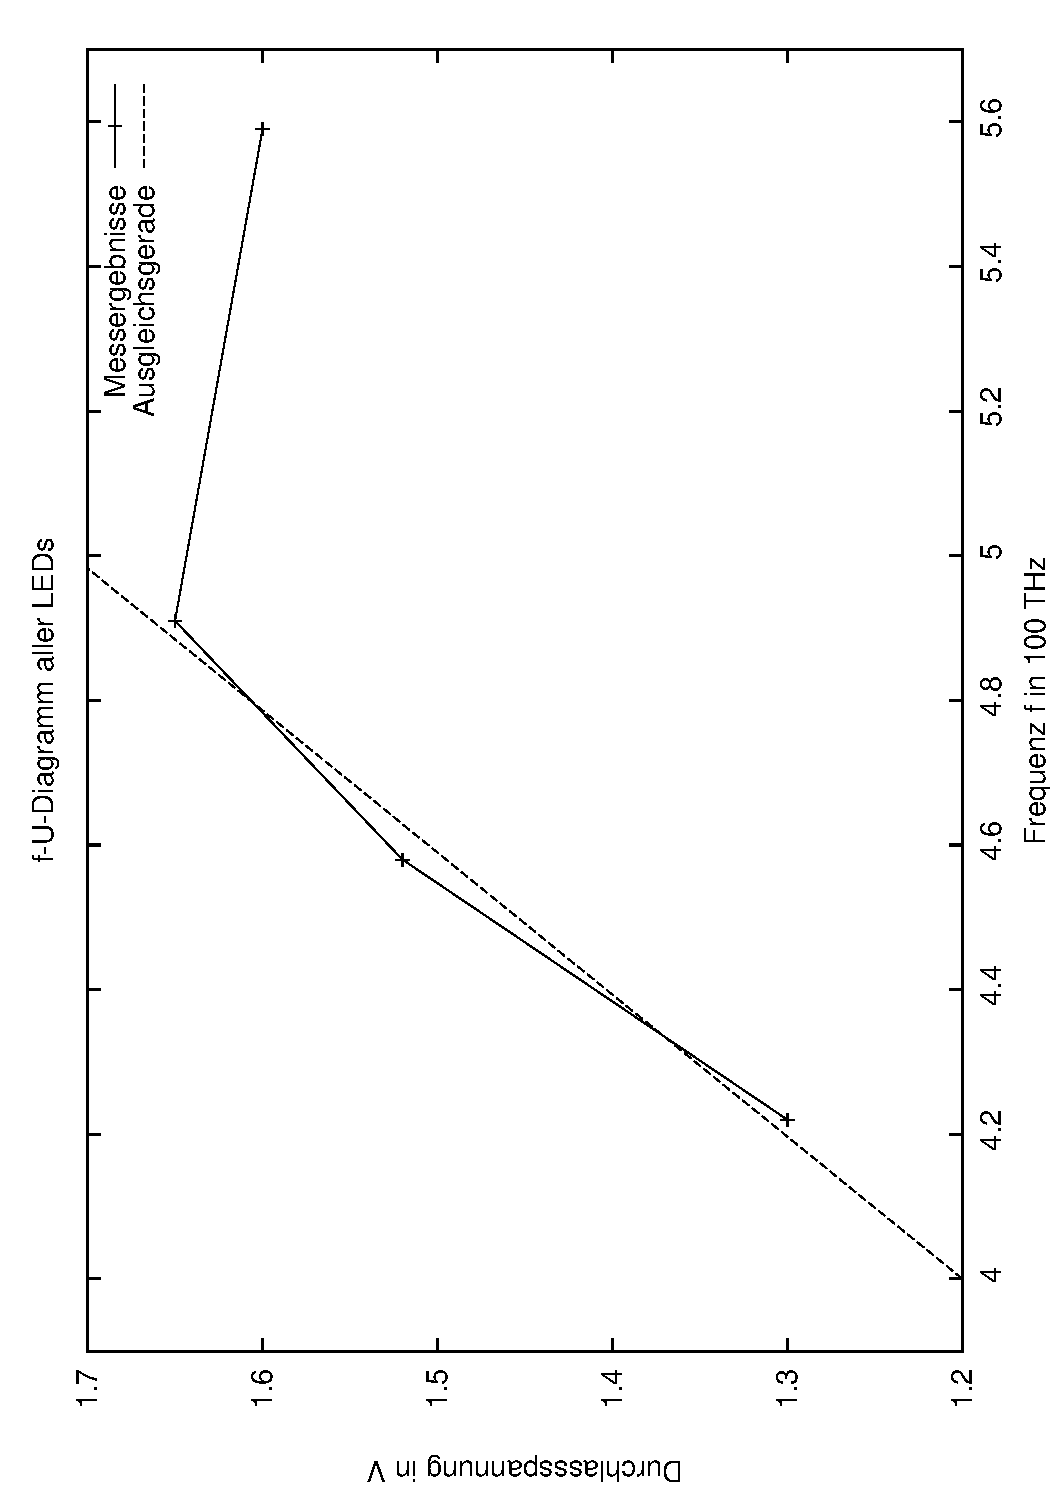
\includegraphics[height=\textwidth,angle=-90]{praktika/mat_praktika/fu_plot01}
   \caption{Ein $f$-$U_D$-Diagramm der LEDs}
   \label{abb_fu}
\end{figure}



\subsection{Fehlerquellen}



\begin{itemize}
   \item Vermutlich haben wir einfach die Distanz vom Gitter zum "`Schirm"' falsch bestimmt: Bspw. ergibt sich für $a_2 = 120cm$ eine durchschnittliche Abweichung von $1,51\%$.
   \item Dadurch dass wir digitale Messinstrumente vewendet haben, könnte es gut sein, dass bei einer bestimmten Spannung schon ein Strom floss, dieser aber nicht angezeigt werden konnte, weil die Zahl so klein war, dass sie hinter dem Komma "`verschwand"' -- dass wir diesen Strom also schlicht nicht ablesen konnten
   \item Das Licht der LEDs ist keinesfalls völlig monochromatisch -- das Maximum hatte schon einen "`Regenbogenrand"' der auf Zerlegung mehrerer Farben hindeutet. Den Abstand der Maxima so zu bestimmen war nicht ganz einfach.
   \item Beim Festsetzen der Klammern zum Markieren der einzelnen Maxima war ein Versuchsteilnehmer auf den anderen angewiesen: Einer beobachtete und dirigierte, der andere stellte ein. Verrutschte der Beobachter, so wurde die Messung zunehmend ungenau, weil sich so auch die Punkte der subjektiv wahrgenommenen Maxima verschoben.
   \item Bei dem Aufbau verrutschte Der Ständer der Diode beim wechseln der einzelnen Dioden -- die Abstände sind weniger genau
   \item Zur Bestimmung verwenden wir eine Näherung (erste \textsc{Fraunhofer}'sche Näherung) -- deswegen können unsere Versuchsergebnisse nicht völlig korrekt sein
   \item Widerstände in den Leitern verfälschen die Spannungsmessung: An der Sperrschicht in der Diode fällt weniger Spannung ab, als wir messen.

\end{itemize}




%\begin{appendix}

\section{Leuchtdioden, Photodioden \& Photozellen}


\paragraph{Leuchtdiode}

Eine Leuchtdiode [...] ist ein elektronisches Halbleiter-Bauelement. Fließt durch die Diode Strom in Durchlassrichtung, so strahlt sie Licht, Infrarotstrahlung oder auch Ultraviolettstrahlung mit einer vom Halbleitermaterial abhängigen Wellenlänge ab. [...]

Der Halbleiter einer LED bildet eine Diode. Durch Anlegen einer Spannung in Durchlassrichtung wandern Elektronen zur Rekombinationsschicht am p-n-Übergang. Auf der n-dotierten Seite bevölkern sie das Leitungsband, um nach Überschreiten der Grenzfläche auf das energetisch günstigere p-dotierte Valenzband zu wechseln, sie rekombinieren mit den dort vorhandenen Löchern. Bei Silizium-Dioden erfolgt der Übergang strahlungslos durch Phononenanregung, indem das Gitter den Impuls der Teilchen aufnimmt. Der direkte Übergang bei Gallium-Arsenid (GaAs) geht mit der Aussendung eines Photons einher. Ein weiterer Ursprung der Photonen besteht in einer plasmonisch-polaronischen Wechselwirkung, die durch einen spinfreien Übergang direkt zur Emission eines Auger-Photoelektrons führt. Dieser Mechanismus spielt insbesondere bei excitonischer Emission in grünen GaP-Leuchtdioden eine Rolle.  --- Quelle: \textsc{Wikipedia}




\paragraph{Fotodiode}

Photodioden sind Halbleiter-Dioden, die sichtbares Licht, in manchen Ausführungen auch IR-, UV- oder Röntgenstrahlen, an einem p-n-Übergang oder pin-Übergang durch den Inneren Fotoeffekt in einen elektrischen Strom umwandeln. Sie werden unter anderem verwendet, um Licht in ein Spannungssignal umzusetzen, oder um mit Licht übertragene Informationen weiterverarbeiten zu können. [...]

Treffen Photonen auf das Material der Diode, so werden in der Raumladungszone Ladungsträger (Elektron-Loch-Paare) erzeugt, was zu einem Stromfluss führt, da die Ladungsträger durch die Diffusionsspannung in die jeweils entgegengesetzt dotierten Zonen wandern. Die Photonen müssen eine höhere Energie als die des Bandabstandes aufweisen, um diesen Effekt hervorzurufen (bei Silizium z. B. mehr als \(1,1 eV\)). Der Fotostrom ist über viele Größenordnungen linear zum Lichteinfall, wenn keine Sättigung eintritt. Im Idealfall trägt jedes Lichtquant, das eine Energie besitzt, die größer als die charakteristische Energielücke (Bandabstand) des Halbleiters ist, zum Stromfluss bei. Praktisch ist der Wert jedoch kleiner und wird als Quantenausbeute bezeichnet. Die Reaktionszeit ist bei geeigneter Beschaltung sehr kurz; sie kann bis herab zu Bruchteilen einer Nanosekunde betragen.
Auch bei Dunkelheit fließt ein temperaturabhängiger, kleiner Strom - der sog. Dunkelstrom (\(I_D\)). Die Dunkelstromkennlinie ist ein wichtiges Qualitätsmerkmal von Fotodioden.  --- Quelle: \textsc{Wikipedia}



\paragraph{Fotozelle}

Eine Fotozelle [...] ist ein Strahlungsdetektor. Sie zählt insofern zu den Elektronenröhren, als sich auch bei ihr in einem evakuierten Glasgefäß eine Anode und eine Kathode (Fotokathode) befinden.

Die Fotokathode besteht aus einem Metall (z.B. Caesium mit besonders geringer Austrittsarbeit), aus dem durch Licht Elektronen freigesetzt werden können (Äußerer Fotoelektrischer Effekt).
 

Ist zwischen Anode (+) und Kathode (-) eine Spannung angelegt, so werden die vom Licht freigesetzten Elektronen zur Anode hin beschleunigt, ein elektrischer Strom (Fotostrom) kann gemessen werden. Ist die angelegte Spannung klein, so ist der Fotostrom proportional zur angelegten Spannung, der Proportionalitätsfaktor hängt von der Belichtungsintensität ab. Dieser Fotostrom geht bei höheren Spannungen in eine Sättigung über, d.h. der Strom steigt bei weiterer Erhöhung der angelegten Spannung nicht weiter an. Dies liegt daran, dass bei geringen Spannungen die elektrische Feldstärke nicht ausreicht, um alle durch den Fotoeffekt an der Kathode austretenden Elektronen in Richtung Anode zu beschleunigen und damit zum Fotostrom beitragen zu lassen. Allerdings können natürlich nicht mehr Elektronen zwischen Kathode und Anode fließen als durch das Licht freigesetzt werden, weshalb die Sättigung auftritt. Auch wenn keine Spannungsquelle mit der Fotozelle verbunden ist, bildet sich zwischen Anode und Kathode bei Belichtung eine Spannung aus - die Anode lädt sich negativ auf. Diese Spannung ist proportional zur Frequenz des eingestrahlten Lichts und kann zur Ermittlung des Planckschen Wirkungsquantums genutzt werden.

Die Spannung bildet sich aus, weil das Licht (genügend hohe Frequenz und damit Energie vorausgesetzt) Elektronen aus der Fotokathode herausschlägt. Diese Elektronen besitzen eine Energie, die der Differenz zwischen Quantenergie des Lichtes und Austrittsarbeit des Elektrons aus dem Kathoden-Metall entspricht. Die freien Elektronen treffen (teilweise) auch auf die Anode und laden diese negativ auf. Dadurch bildet sich eine elektrische Spannung zwischen den Elektroden aus. Weitere Elektronen müssen nun das sich ausbildende elektrische Feld durchlaufen, um auf die Anode aufzutreffen, wozu sie Energie benötigen. Schließlich ist die Spannung so groß, dass die Energie der neu herausgelösten Elektronen nicht mehr ausreicht, die Platte zu erreichen - die Spannung bleibt konstant.  --- Quelle: \textsc{Wikipedia}









%\end{appendix}







% 
% 
% \end{document}
